\documentclass[conference]{IEEEtran}
\usepackage{cite}
\usepackage{amsmath,amssymb,amsfonts}
\usepackage{algorithmic}
\usepackage{graphicx}
\usepackage{textcomp}
\usepackage{xcolor}
\usepackage{fancyhdr}
\usepackage[hyphens]{url}

\def\BibTeX{{\rm B\kern-.05em{\sc i\kern-.025em b}\kern-.08em
    T\kern-.1667em\lower.7ex\hbox{E}\kern-.125emX}}

% Ensure letter paper
\pdfpagewidth=8.5in
\pdfpageheight=11in


%%%%%%%%%%%---SETME-----%%%%%%%%%%%%%
\newcommand{\iscasubmissionnumber}{NaN}
%%%%%%%%%%%%%%%%%%%%%%%%%%%%%%%%%%%%

\fancypagestyle{firstpage}{
  \fancyhf{}
\renewcommand{\headrulewidth}{0pt}
  \fancyhead[C]{\normalsize{ISCA 2021 Submission
      \textbf{\#\iscasubmissionnumber} \\ Confidential Draft: DO NOT DISTRIBUTE}} 
  \fancyfoot[C]{\thepage}
}  


\pagenumbering{arabic}

%%%%%%%%%%%---SETME-----%%%%%%%%%%%%%
\title{O4: Learning a Dynamic Phase Ordering Policy} 
\author{Ajay Uppili Arasanipalai}
%%%%%%%%%%%%%%%%%%%%%%%%%%%%%%%%%%%%

\begin{document}
\maketitle
\thispagestyle{firstpage}
\pagestyle{plain}



%%%%%% -- PAPER CONTENT STARTS-- %%%%%%%%

\begin{abstract}

  Phase ordering, the task of choosing and ordering code transformations from a
  set of semantics-preserving passes, is an important problem for optimizing
  compilers. The ordering of passes can have a significant impact on key
  performance metrics for the generated code, such as instruction count, run
  time, and build time.

  In this work, we propose a dynamic phase ordering policy based on a learned
  cost model for LLVM passes. Our learned cost model is able to predict code
  size reduction with a 9.5\% error rate. We show that our cost model can be
  used to generate phase ordering policy that outperforms LLVM's built-in
  \texttt{-Oz} policy.

  Code and pretrained models can be found at \url{https://github.com/iyaja/O4}.

\end{abstract}

\section{Introduction}

The LLVM \cite{lattner2004llvm} compiler framework has become a widely
successful and popular tool for building optimizing compilers by abtracting away
the front-end and back-end to enable powerful language-agnostic tools to be
built over LLVM intermediate representation (IR).

Among the most useful tools in LLVM is \texttt{opt}, an optimization engine
that transforms LLVM IR code by applying a set of transformations called passes,
such as dead code elimination, constant propagation, and loop unrolling. These
passes can, in general, be ordered arbitrarily, and the order of the passes can
have a significant impact on the performance of the generated code. There are
many phase ordering a classically challenging problem.

\textbf{Complex Complier Internals.} LLVM passes can be complex. Some involve
many thousands of lines of C++ code designed by human experts with complex
heuristics. Designing a good phase ordering policy involves not only
understanding how each of these passes work, but also how specifically on the IR
to be optimized.

\textbf{Large Search Space.} The search space of all possible optimization
pipelines is very large (arguably infinite). For a pipeline with \(n\) phases
and \(m\) passes, the search space is \(O(n^m)\) - exponential in the number of
phases. Furthermore, there is no hard limit to the total number of phases that
can be used in a pipeline, but there is a point of diminishing returns. Applying
more passes does not nessecarily improve performance, and can sometimes even
hurt it. Furthermore, using more passes also increases build time, meaning a
complex pipeline that improves performance but has too many passes may be
unprofitable. A good policy must be able to balance the trade-off between
performance metrics and build time.

\textbf{Interdependancies Between Passes} While phase ordering can be modeled as
a sequential decision making process, passes in LLVM serve various purposes and
can have complex interdependencies. For example, while some passes may not have
an immediate or appreciable effect on the generated code, they may enable other
passes to be applied or work more effectively.

Currently, LLVM implements a collection of "good default" optimization policies,
such as \texttt{-O0} (no optimization), \texttt{-O1} (some level of runtime
reduction with quick builds), \texttt{-Os} (codesize reduction), \texttt{-Oz}
(aggresive codesize reduction), and \texttt{-O3} (aggresive runtime reduction).
This is by far the most common approach for optimizing compilers.

Additionally, LLVM's built-in optimization pipelines are static - they apply the
same set of passes to all IR. This is potentially suboptimal, as certain
optimizations may be more or less effective on certain code patterns. However,
designing a dynamic phase ordering policy is sufficiently complex that it is not
feasible write manually. LLVM's default pipelines have been emperically shown to
work well across a wide range of code patterns, and we argue that this reliance
on experimental data naturally suggests that a learning-based search method
might be more effective.

\section{Method}

In this work, we focus on the problem of choosing a dynamic phase ordering that
minimizes codesize. Here, we present our proposed method for building and
training O4 (collectively referring to both a cost model and the phase ordering
policy). Our approach can be broken down into three steps:

\begin{enumerate}
  \item Train a cost model to predict instruction count.
  \item Train a classifier to predict the optimal pass to apply to current IR,
        using the cost model as a loss function.
  \item Run the trained policy recursively on the desired IR, applying passes
        sequentially after each forward step.
\end{enumerate}

The following sections decribe each of these steps in more detail.

\subsection{Training a Cost Model}

The first component of O4 is a cost model that predicts the effect of applying a
given optimization from LLVM's predefined set of 124 passes exposed in Compiler
Gym \cite{CompilerGym}.

We use a transformer-based architecure for the cost model. More details are
provided in \ref{sec:neural_network}.

We use the LLVM IR instruction count as a target metric. While it is not a
measure of true codesize reduction, as it does not take into account the effects
of lowering, it is fast to evaluate, deterministic, and platform-independent.
Additionally, IR instruction count is the default reward metric used in Compiler
Gym \cite{CompilerGym}, enabling us to draw a fair comparison with similar
methods that have been evaluated on the same dataset and benchmarks.


The approach is summarized in \ref{fig:training_cost_model}.

\label{fig:training_cost_model}
\begin{figure}
  \centering
  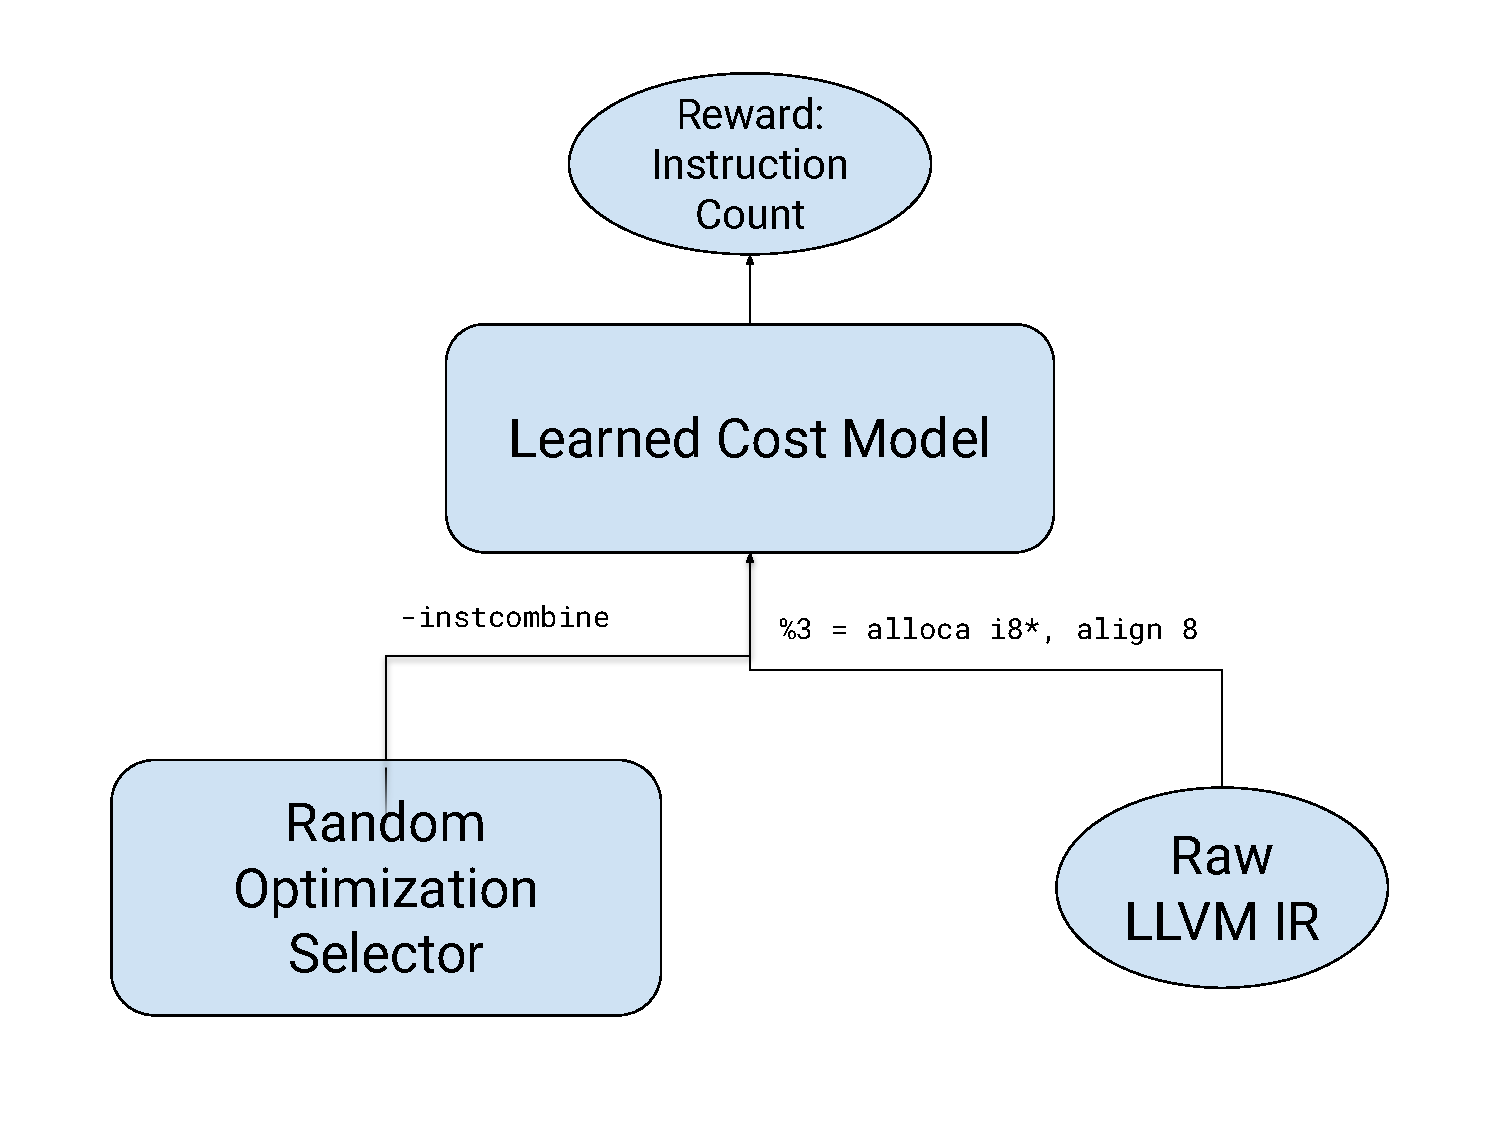
\includegraphics[scale=0.3]{figures/training_1.pdf}
  \caption{\textbf{Training the cost model.}}
\end{figure}

The cost model is trained using a supervised learning. Since the true reward
(instruction count after applying an optimization pass to IR) is known at
training time, we simply train the cost model to minimize the mean squared error
between the true reward and the predicted reward.

The differentiable cost model learns predict the result of applying a given
transformation to a given IR. The cost model takes the raw LLVM IR as input and
predicts the desired reward metric, as shown in \ref{fig:training_cost_model}.

The groud truth reward signal, which the cost model attempts to approximate, is
the reduction in instruction count relative to LLVM's built-in \texttt{-Oz}
pipeline:

\[ R = \frac{IC_{o0} - IC_{o \sim \mathcal{U}(A)}}{IC_{o0} - IC_{oz}} \]

Where \(IC_p\) is the LLVM IR instruction count of the program after applyng
optimization pipeline \(p\) (obtained using the \texttt{IrInstructionCount}
observation space in Compiler Gym).

\subsection{Training a Policy Network}

Once the cost model has been trained, we can use it to train a classifier that
predicts which optimization pass to apply to a given IR. The optimization
prediction network takes the raw LLVM IR as input and predicts which one among
the 124 passes should be applied. Then, the cost model is used as a supervision
signal to train the network to improve it's predictions.

Since the cost model is a differentiable function, we can backpropagate through
it and treat it as a loss function, with the learning objecttive of the policy
network being to minimize the estimated instruction count from the cost model.

This second training step is summarized in \ref{fig:training_policy_network}.

\label{fig:training_policy_network}
\begin{figure}
  \centering
  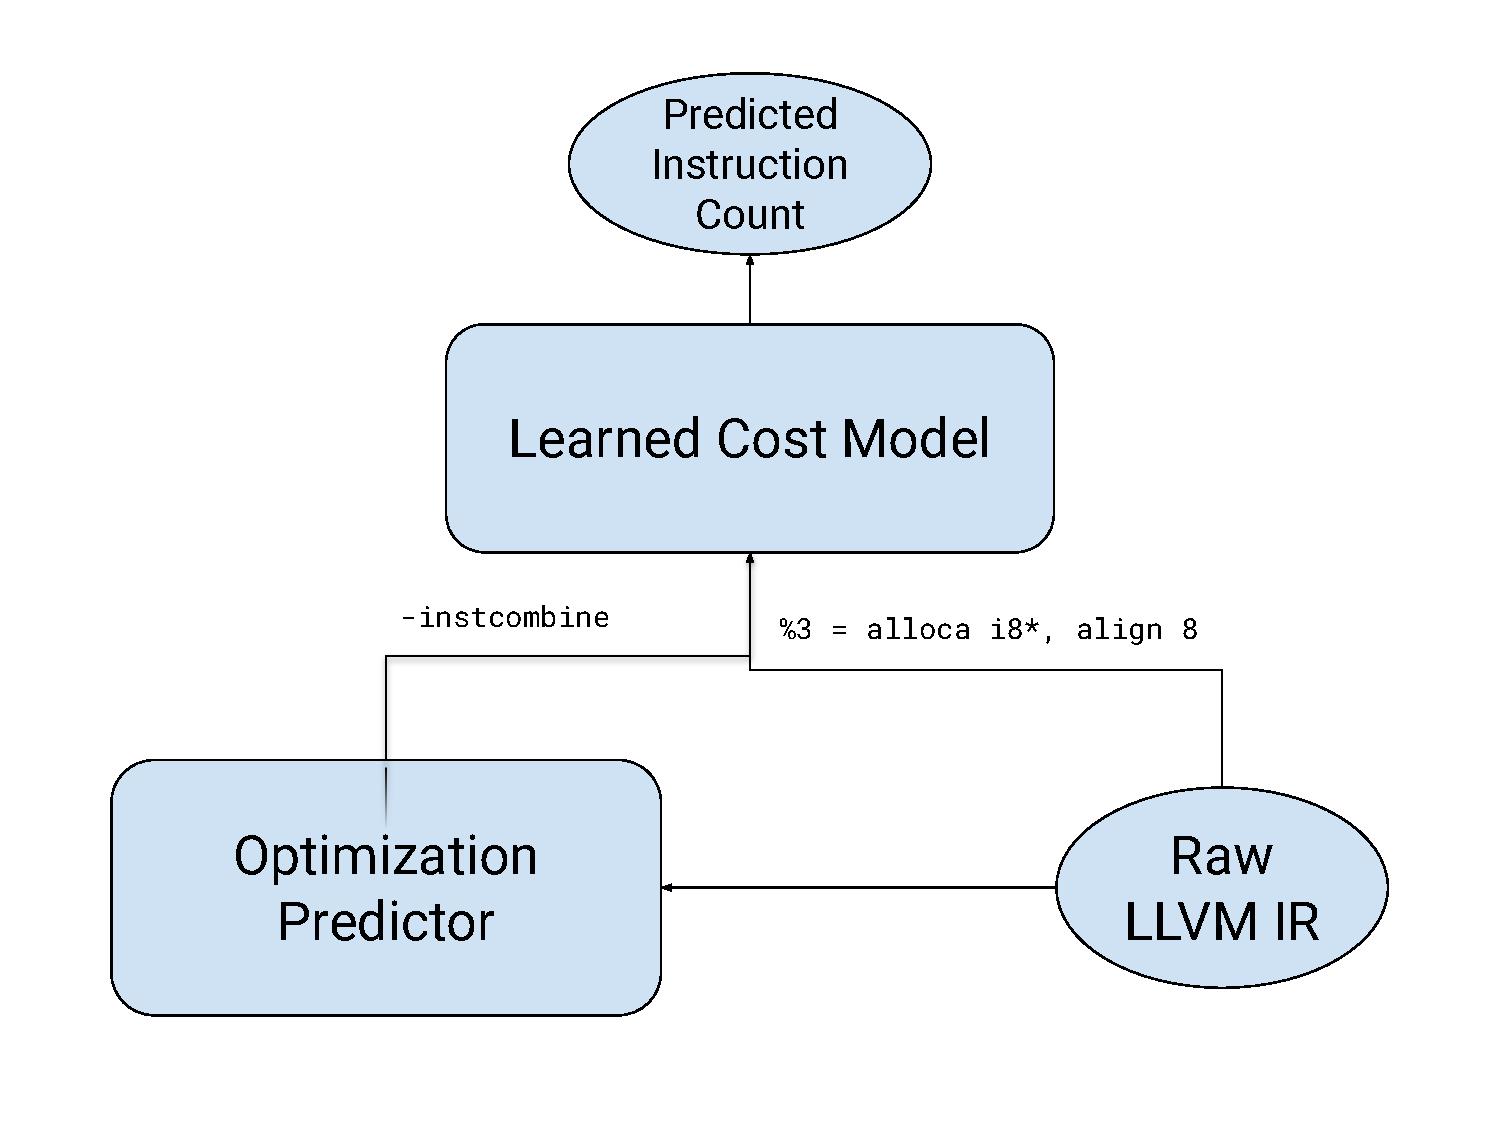
\includegraphics[scale=0.3]{figures/training_2.pdf}
  \caption{\textbf{Training the policy network.}}
\end{figure}

\subsection{Generating a Phase Ordering}

With both models trained, the final step is to generate a dynamic phase
ordering. This is done by applying the policy network to the raw LLVM IR
recurrently - apply the optimization predicted by the policy network, and then
pass the transformed IR back into the network to predict the next optimization.
This process repeated recurrently until the desired target performace is
reached.

As shown in \ref{fig:inference}, the only model required at compile time is a
single copy of the optimization predictor. The cost model can be discarded once
optimization predictor as been trained and does not need to be integrated into
the compiler, unlike in other machine learning methods. This simple functional
interface makes it easy to integrate O4 into existing compiler frameworks
without rewriting pass managers to use the cost model directly.

\label{fig:inference}
\begin{figure}
  \centering
  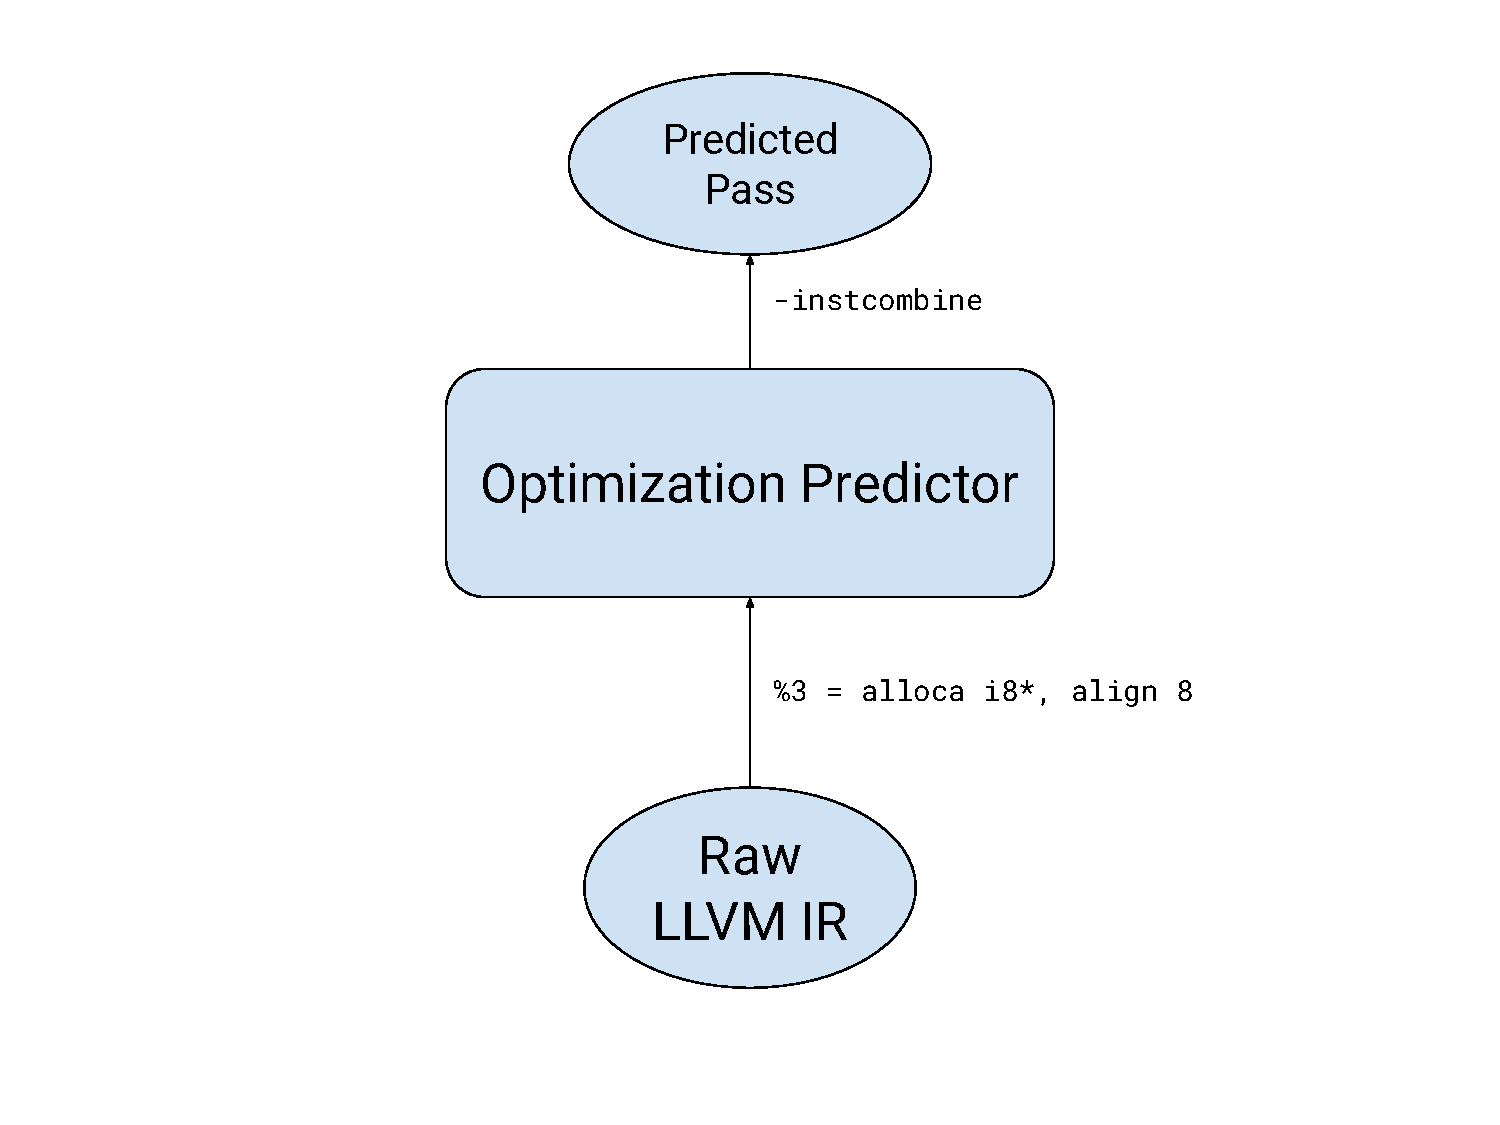
\includegraphics[scale=0.3]{figures/inference.pdf}
  \caption{\textbf{Generating a phase ordering.}}
\end{figure}

\section{Implementation}

Next, we describe the implementation and training details of O4. Code is
available in at \url{https://github.com/iyaja/O4}.

\subsection{Inputs and Data}

We train our models using a representative subset of datasets built into
Compiler Gym \cite{CompilerGym}. Specifically, we use a combination of programs
from the NASA parallel benchmark suite \cite{bailey1995parallel} and cBench
\cite{fursin2009collective}. Unfortunately, due to the use of this custom subset
of small programs and limited compute resources, we cannot make a fair
comparison with current approaches on the Compiler Gym leaderboards.

The datasets are exposed as raw human-readable LLVM IR in Compiler Gym, and we
use a custom tokenizer based on WordPiece \cite{devlin2018bert} and Inst2vec
\cite{ben2018neural} for our preprocessing pipeline. We train the WordPiece
tokenizer on our dataset that is first normalized and preprocessed by Inst2vec
\cite{ben2018neural}. We do \textbf{not} use the embeddings or tokens from
Inst2vec, and instead build a custom fast tokenizer to work with the Huggingface
Transformers library \cite{wolf2019huggingface} and retrain the RoBERTa's
embedding layer instead of using Inst2vec's fixed 200-dimensional vectors.

Where possible, the tokenizer learns to group entire instructions into a single
token. This enables us to pack many more instructions into an input sequence
than a conventionally trained Byte-Pair Encoding (BPE) tokenizer, which is
especially important for models like RoBERTa, which have an input sequence
length limit of 512 tokens. Since the model is trained to predict instruction
count, not including all instructions can be problematic, since the model would
have no sense of how long the full IR is. Future work could investiage
augmenting the raw IR with additional metadata to circumvent this limitation.

For the cost model, the current pass to be applied on the is prepended as a
special token to the input sequence, For the policy network, the tokenized
instructions are passed directly to the transformer.

\label{sec:neural_network}
\subsection{Neural Networks}

We use RoBERTa \cite{liu2019roberta}, a popular variant of the BERT
\cite{devlin2018bert} transformer model  as our base architecture for both the
cost model and the policy network. We initialize it from the CodeBERT
\cite{feng2020codebert} checkpoint and leave architecure exploration for future
work, acknowleding that there is potentially scope for more complex model that
use , such as Programl embeddings \cite{cummins2020programl} with graph neural
networks to extract more semantic information from the IR.

CodeBERT \cite{feng2020codebert} is a large language model pretrained on a large
dataset of code snippets in high level languages, such as Java and Go. While
this is not representative of our target domain (LLVM IR), we reasoned that it
would be better than initializing our cost model from random weights and
pretraining a new language model from scratch. While pretraining a language
model on raw LLVM IR is bound to be a more effective, this approach was
prohibitively expensive, and we leave it for future work.

Both the cost model and the policy network are implemented using the Huggingface
Transformers library \cite{wolf2019huggingface}. Pretrained models and are
available on the Huggingface model hub \footnote{Pretrained models and
  tokenizers are availabe at https://huggingface.co/iyaja/O4}.

\section{Results}

Our current results are summarized in \ref{table:results}. Of main interest is
the error rate of the cost model - the best model, trained on 1000 samples of
cBench \cite{fursin2009collective}, is able to predict the relative instruction
count reduction with an error rate of 11.4\% (root mean-squared error).

\begin{scriptsize}
  \begin{table}[h!]
    \begin{center}
      \caption{Summary of results.}
      \label{table:results}
      \begin{tabular}{|l|l|l|l|l|}
        \hline
        \textbf{Dataset} & \textbf{\begin{tabular}[c]{@{}l@{}}Unique \\
            Programs\end{tabular}} & \textbf{Samples} & \textbf{Passes} &
        \textbf{MSE}                                                                                     \\ \hline
        cbench-v0        & 23                                     & 100              & 5
                         & 0.031                                                                         \\ \hline
        cbench-v0        & 23                                     & 500              & 10
                         & 0.019                                                                         \\ \hline
        cbench-v0        & 23                                     & 1000             & 20              &
        \textbf{0.013}                                                                                   \\ \hline
        npb-v0           & 122                                    & 64               & 32
                         & -                                                                             \\ \hline
      \end{tabular}
    \end{center}
  \end{table}
\end{scriptsize}

Unfortunately, the policy network network, as trained on the best cost model, is
unable to reach the performance of random search. We hope to iterate on this
model an improve it's performance in future work.


\section{Conclusion}

Phase ordering is an import yet complex classic compiler problem that can have a
significant impact on key performance metrics for the generated code. Our
proposed method, O4, uses a learned cost model to generate a dynamic phase
ordering policy. While our generated phase orderings do not outperform LLVM's
built-in \texttt{-Oz} policy on average, they demonstrate that a learned policy
for phase ordering, with more training data and time, can be effective.

Furthermore, our approach learns and adapts and scales with more data, which
opens the door to phase ordering policies finetuned for specific domains,
architecures, and applications.

% \section*{Acknowledgements}
% This document is derived from previous conferences, in particular ISCA
% 2019, MICRO 2019, ISCA 2020, and MICRO 2020.

%%%%%%% -- PAPER CONTENT ENDS -- %%%%%%%%


%%%%%%%%% -- BIB STYLE AND FILE -- %%%%%%%%
\bibliographystyle{IEEEtranS}
\bibliography{refs}
%%%%%%%%%%%%%%%%%%%%%%%%%%%%%%%%%%%%

\end{document}

